\documentclass[10pt,a4paper]{article}
\usepackage[utf8]{inputenc}
\usepackage{amsmath}
\usepackage{amsfonts}
\usepackage{amssymb}
\usepackage{graphicx}
\usepackage{color}
\usepackage{float}
\usepackage[dutch]{babel}
\usepackage{eurosym}
 
\definecolor{codegreen}{rgb}{0,0.6,0}
\definecolor{codegray}{rgb}{0.5,0.5,0.5}
\definecolor{codepurple}{rgb}{0.58,0,0.82}
\definecolor{backcolour}{rgb}{0.95,0.95,0.92}
\usepackage{listings}
\lstdefinestyle{cstyle}{
    backgroundcolor=\color{backcolour},   
    commentstyle=\color{codegreen},
    keywordstyle=\color{magenta},
    numberstyle=\tiny\color{codegray},
    stringstyle=\color{codepurple},
    basicstyle=\footnotesize,
    breakatwhitespace=false,         
    breaklines=true,                 
    captionpos=b,                    
    keepspaces=true,                 
    numbers=left,                    
    numbersep=5pt,                  
    showspaces=false,                
    showstringspaces=false,
    showtabs=false,                  
    tabsize=2
}
\graphicspath{ {./images/} }

\begin{document}
\begin{titlepage}
    \centering
    \vfill
    {\Large
    Swarming\\
   
    {\small Research framework}\\
        
        \vskip2cm
        {\small M. van Wilgenburg, W. Mukhtar, E. van Splunter, M. Siekerman, T. Zaal and M. Visser}\\
    }    
    \vfill
%    \includegraphics[width=1\textwidth]{WireS4}
    
    \vfill
    \vfill
\end{titlepage}

\newpage

\tableofcontents
\newpage


\section{Problem analysis}
Researcher have always been inspired by nature. When they looked at "social" insects like ants they discovered "swarming"\cite{swarmwiki} . The behaviour of one ant on its own seems illogical, but together they solve problems of great importance for the entire colony. These ants make us of the so called "trail laying" and "trail following" principle. Every ants lays a trail of pheromones, when a few ants walk back and forth to a food source. The one walking the shortest route will lay a more concentrated trail. The other ants will get attracted by the strongest trail, this way a positive feedback loop is created, which will make every ant walk the shortest route if given enough time. This is one example where relatively simple units, can achieve complex goals like path finding because they work together in a swarm. This principle is called "swarm intelligence"\cite{swarmintelligence}.

Swarming can have alot of up sides compared to the "classical" approach. A few are: quicker solution time, lower unit complexity and a greater fault tolerance\cite{swarmintelligence}. When for example one of the units breaks down, then will the other units still be able to complete the task. When this happens to one, more complex unit, this wont be the case. For these reasons its interesting to researching the applications of swarming.



\section{Context analysis} 
The Delft university of technology started a program to research the applications of swarming. In this program multiple universities work together to make this research possible. The idea of this program is that each project group contributes a small bit to reach the end result, which will be a working swarm of robots. The technology developed should be modular, so it can be easily used on other platforms.\\The programs focus lies on researching the applications of swarming on Mars. Its preferable that the technologies developed also work on Mars, but in some cases other technologies can be used to cut the cost. For example, for a simple proximity sensor on earth, an ultrasonic sensor would do just fine. But in the Mars atmosphere the ultrasonic waves get heavily dampened to the point where the sensor just wont work\cite{soundonmars}. The cheapest sensor that would work on Mars would be a lidar\cite{lidarmars}. While the average ultrasonic sensor costs around 2 \euro the cheapest lidar costs atleast 100 \euro. In this project the aim is to build one unit for around 200\euro, just one lidar sensor would be half of the robots budget. To proof the concept of swarming the robots don't need to be "Mars proof", so costs will be cut where possible.\\

\section{Problem definition}
Swarming intelligent systems are typically made up of simple agents(robots) interacting locally with one another and their environment. The group of individuals acting in such manner is referred to as a swarm\cite{swarmintelligence}. For a group of robots to qualify as a swarm-robotics the following criteria have to be met:

\begin{itemize}
    \item Autonomy – It is required that the individuals that make up   the swarm-robotic system are autonomous robots. They are able to        physically      interact with the environment and affect it.
    \item Large number – A large number of units is required
    as well, so the cooperative behavior (and
    swarm intelligence) may occur. The minimum number
    is hard to define and justify. The swarm-robotic
    system can be made of few homogeneous groups of
    robots consisted of large number of units. Highly heterogeneous 
    robot groups tend to fall outside swarm
    robotics.
    \item Limited capabilities – The robots in a swarm
    should be relatively incapable or inefficien on their
    own with respect to the task at hand.
    Scalability and robustness – A swarm-robotic
    system needs to be scalable and robust. Adding the
    new units will improve the performance of the overall
    system and on the other hand, loosing some units will
    not cause the catastrophic failure.
    \item Distributed coordination – The robots in a swarm
    should only have local and limited sensing and communication
    abilities. The coordination between the
    robots is distributed. The use of a global channel for
    the coordination would influence the autonomy of the
    units.
\end{itemize}

These criteria are a good indication of what makes a system swarm-robotic. But should not be used to determine whether a system is swarm-robotic or not. This is because some criteria are still somewhat phage\cite{swarmintelligence}.

Looking at these criteria we chose to define the problem into two sub-problems. One covers Autonomy, Large number and limited capabilities. And the other Distributed coordination. 

There are multiple aspects that should be taken into account. First the project focus will be building a swarming module. The features of this module will be discussed later. What's important is that the module should be "plug and play". What is meant by this is that the only in and output will be a communication protocol and a power input. This way the module can later be used on different platforms later in the program.\\ Then To properly test the swarming module, a swarm of robots will be need to be developed.

\section{Doelstelling}
In samenwerking met de technische universiteit Delft en de Hogeschool van Amsterdam moet er een zwerm robots (zwerm) worden ontwikkeld die samen een taak uitvoeren. Zwermen is een breed begrip. Daarom wordt hieronder opgesomd, aan welke specificaties voldaan moet worden voordat er over zwermen gesproken mag worden. Tevens zal hieruit een duidelijk doel naar voren komen wat behaald moet worden wat betreft het laten samen werken van verschillende robots binnen een zwerm.

Een groep robots moet aan de volgende eisen voldoen om onder de categorie zwermen te vallen:

\begin{itemize}

\item Autonoom		-	Het is vereist dat de  individuele  robots  binnenin  een  zwerm   
systeem autonoom zijn. Ze moeten tevens over een fysieke interactie beschikken om de omgeving te waarnemen en eventueel aan te passen \cite{swarmintelligence}.

\item Een groot aantal	-	Een groot aantal is ook vereist om het samenwerkende gedrag
te bereiken. Het minimale aantal robots is lastig te definiëren. Een zwerm kan al gecre\"eerd worden met een paar simpele robots\cite{swarmintelligence}.
\item Gelimiteerd	-	De robots in een zwerm moeten individueel relatief incapabel
of ineffici\"ent zijn. Als een individuele robot de gehele taak van
de zwerm kan uitvoeren. Is in dit geval de inzet van de zwerm geheel nutteloos\cite{swarmintelligence}.

\item Schaalbaar		-	Een   zwerm    robots moet   schaalbaar  en   robuust   zijn. Het
toevoegen van nieuwe robots aan het gehele systeem moet de uitvoering van de taak over het geheel verbeteren. Tevens als er verschillende units binnen de zwerm verloren raakt mag dit niet tot catastrofale fouten lijden\cite{swarmintelligence}.

\item Co\"ordinaten	-	De robots   binnen een zwerm  moeten over een  gelimiteerde
communicatie en waarneming beschikken. De coördinaten tussen de verschillende robots gedistribueerd. Het gebruik van en globale communicatie kanaal voor de co\"ordinaten be\"invloed de autonomie van de verschillende units\cite{swarmintelligence}.
\end{itemize}

Het doel is om een zwerm robots te ontwikkelen die voldoen aan de bovenstaande criteria.

\section{Research-question}

The main question of this research is as following: \textit{"How can a minimum  of three robots operate in a swarm".} To give an answer to this question there are multiple subquestions to research first. 
 
%In dit onderzoek wordt de volgende hoofdvraag onderzocht:"Hoe kunnen er minimaal drie robots in een zwerm opereren?". Om de hoofdvraag te kunnen beantwoorden zijn antwoorden nodig op een aantal deelvragen.

\section{Sub-questions} 
The following questions need to be answered to come to a good conclusion to our research:

\begin{itemize}

    \item "What is swarming?"
    \begin{itemize}
        \item "What is the definition of swarming?"
        \item "How many robots are needed to create a swarm?"
        \item "How do the units communicate within the swarm?"
    \end{itemize}    
    \begin{itemize}
        \item "What software protocol should be used?"
        \item "What hardware protocol should be used?"
        \item "What is de minimal required communication speed?"
        \item "What hardware is needed to implement the communication?"
    \end{itemize}
    \item "What methods are there to propel the robot?"
    \begin{itemize}
        \item "What actuators can be used to drive the robot?"
        \item "How would the energy of the actuator be used to make the robot drive?"
        \item "What kind of effectors should be used?"
    \end{itemize}
    \item "What energy supply should be used to distribute the energy in the robot?"
    \begin{itemize}
        \item "How can the energy supply be managed?"
        \item "Is it possible to implement a recharge point?"
        \item "How can the energy supply be handled safely?"
    \end{itemize}
\end{itemize}
\newpage

\section{Specificaties}
In dit document worden de functionele eisen omschreven voor het bouwen van een robot die in samenwerking met andere robots een taak kan uitvoeren, zwermen. De specificaties zijn opgedeeld in verschillende functies waarmee het doel bereikt kan worden. 
Volgens de MoSCow -methode worden de te behalen specificaties op het gebied van zwermen geclassificeerd. De bijbehorende specificaties worden in dit hoofdstuk verder toegelicht. In het blokschema getoond in figuur \ref{fig:blockschematic}, zijn de verschillende modules aan elkaar verbonden. 

\begin{figure}[h]
    \centering
    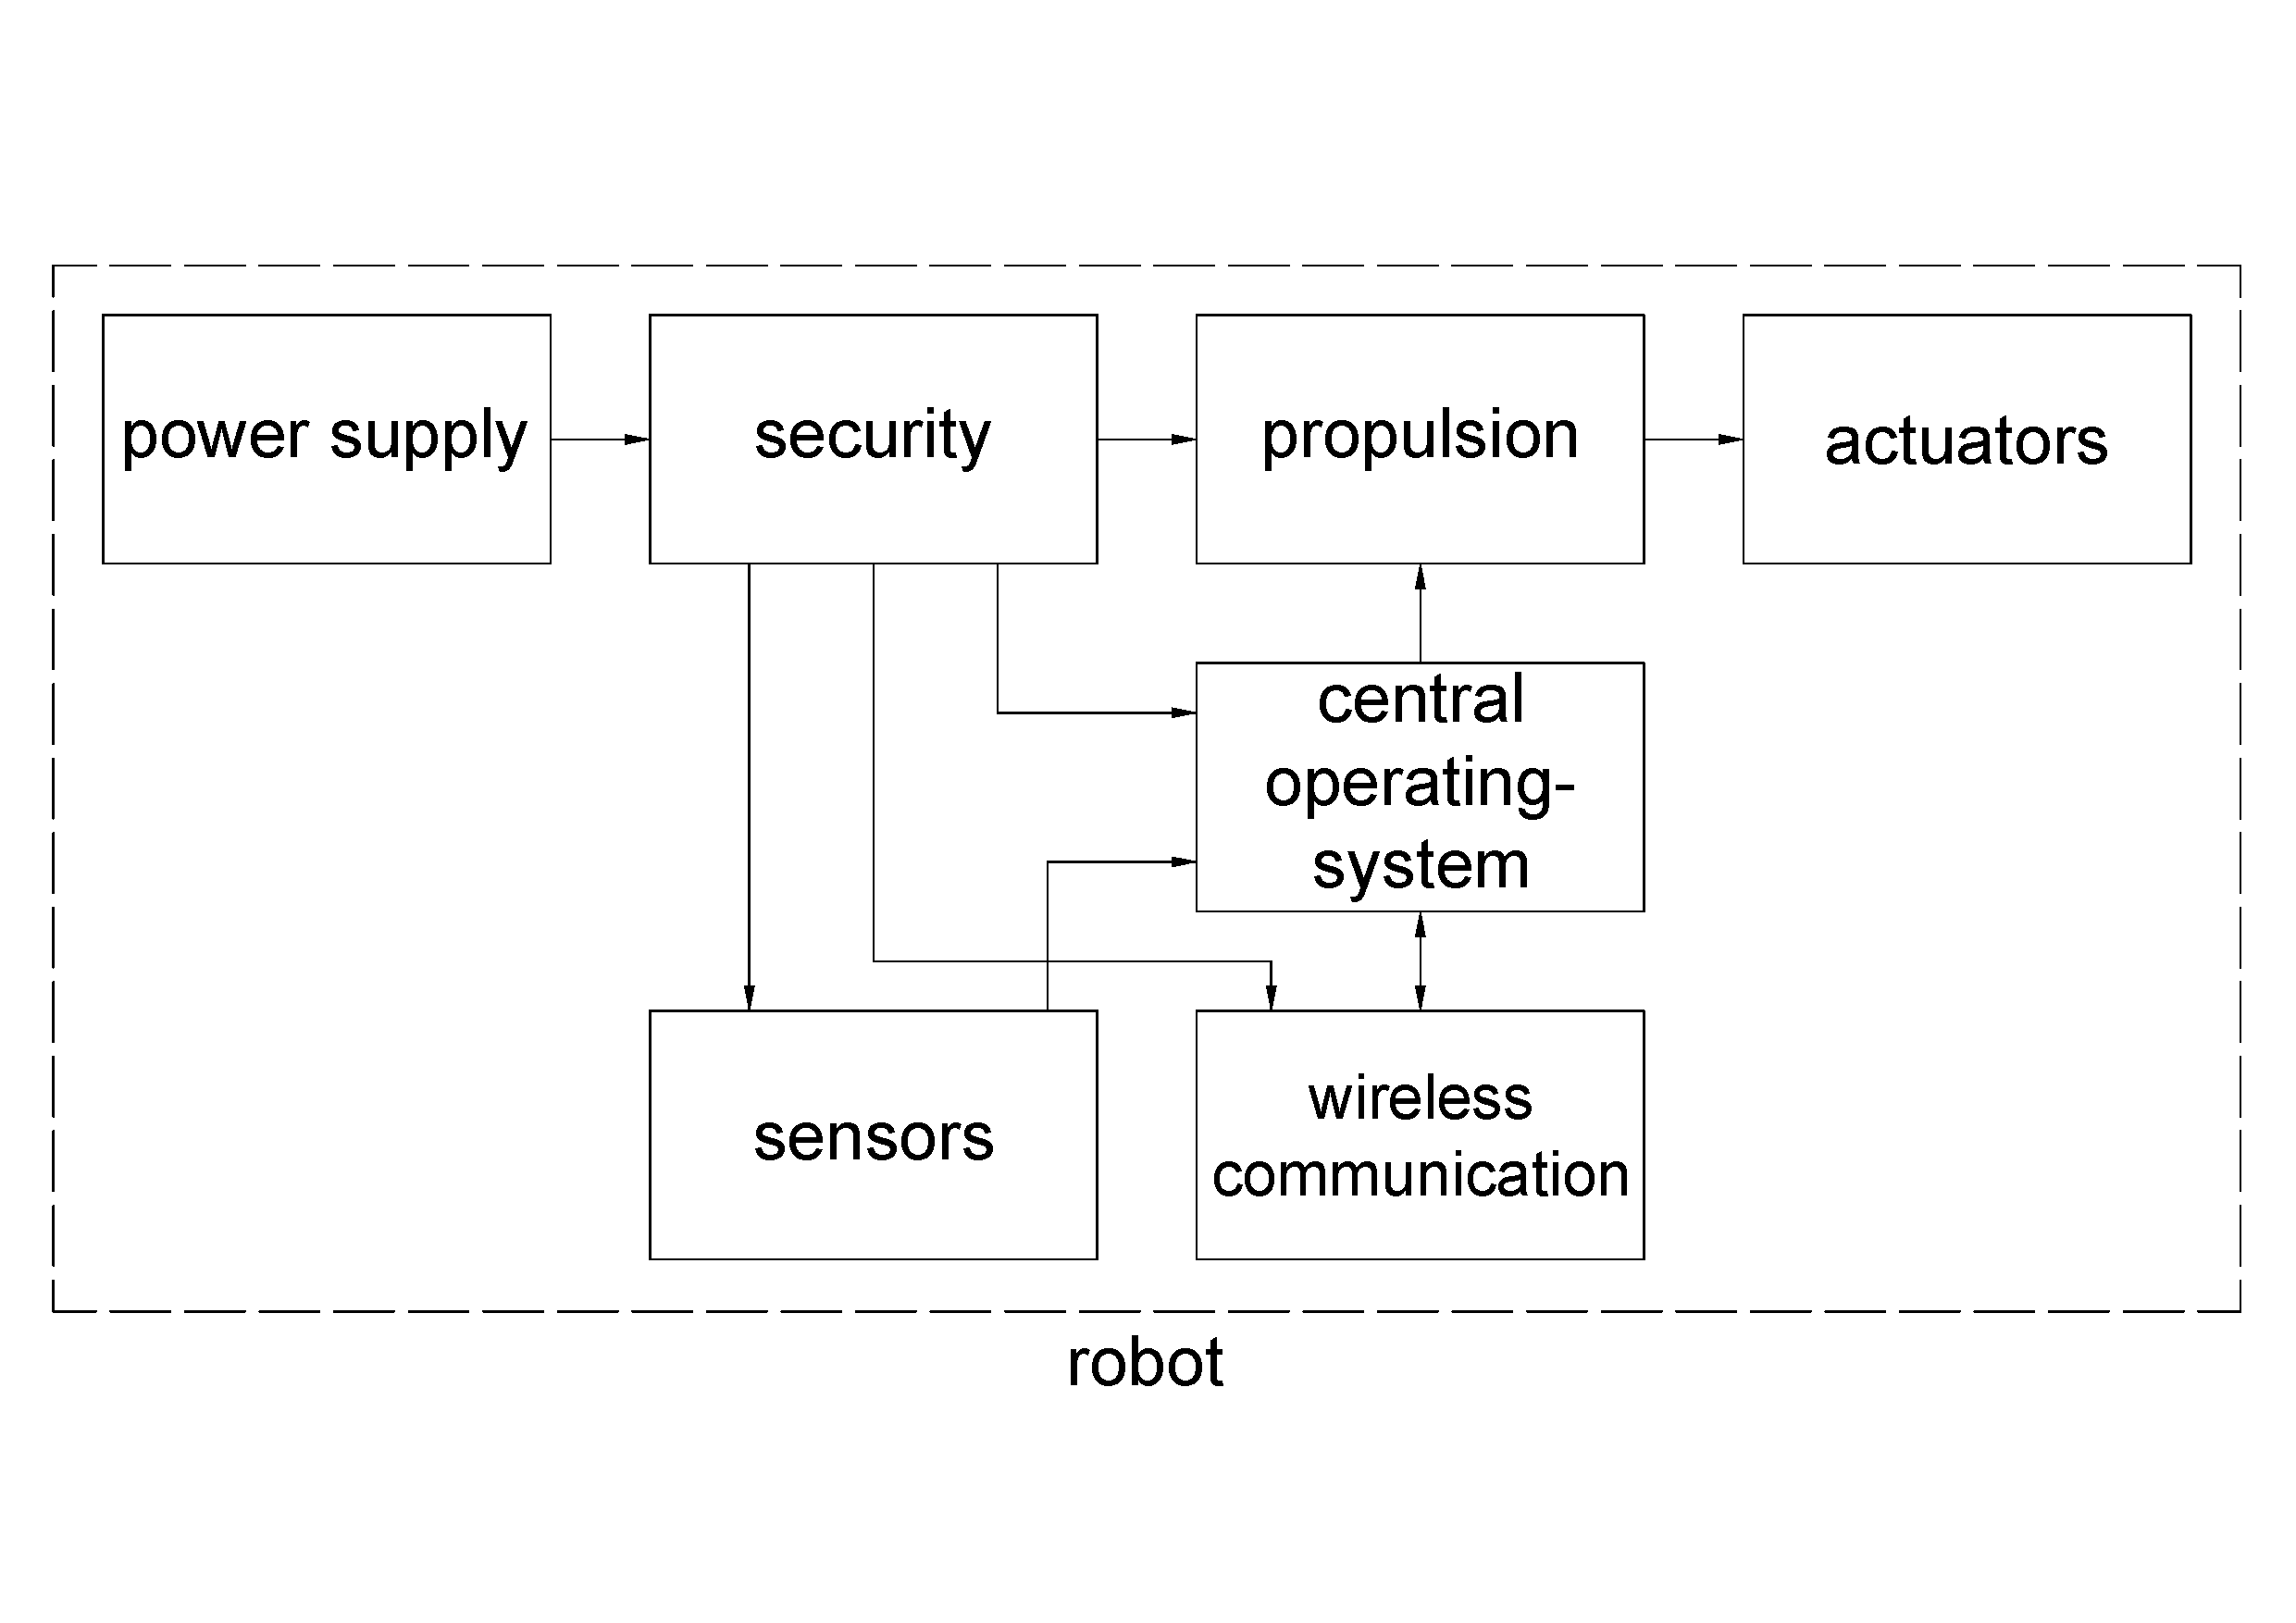
\includegraphics[width=1\textwidth]{blockschematic}
    \caption{Versimpelde weegave in een blokschema van de samenhang van de verschillende deelsystemen binnen de robot.}
    \label{fig:blockschematic}
\end{figure}



\subsection{Must haves}
\begin{itemize}
\item Robots moeten onderling kunnen communiceren
\item De communicatie moet draadloos zijn
\item Iedere module moet zijn eigen energievoorziening hebben
\item De robot moet zichzelf omridirectioneel voort kunnen bewegen
\item Kan met meerdere robots opereren in een zwerm
\end{itemize}

\subsection{Should haves}
\begin{itemize}
\item In staat om een payload te vervoeren
\item Modulaire opbouw van systeem
\end{itemize}

\subsection{Could haves}
\begin{itemize}
\item Kan zich voortbewegen volgens het principe van de ZebRo
\item Mogelijkheid tot zelfstandig opladen/bijladen van energievoorziening
\item Toont een vorm van intelligentie
\item Schaalbaar maken van de zwerm populatie
\item Is er zich van bewust wanneer de robot zich ondersteboven bevind
\item De robot kan zich voortbewegen volgens het principe van de robot
\item De robots moeten modulair zijn
\item De robots kunnen zich opladen in een oplaadstation
\end{itemize}

\subsection{Won't haves}
\begin{itemize}
\item Een master in het zwerm netwerk
\end{itemize}

\newpage

\section{Deelspecificaties}

\begin{table}[H]
\centering
\caption{Sensoren}
\label{Sensoren}
\begin{tabular}{|l|l|}
\hline
Module    & Sensoren \\ \hline
Ingangen  & Communicatie met het systeem             \\ \hline
Uitgangen & Communicatie met het systeem             \\ \hline
Functies   & \begin{tabular}[c]{@{}l@{}}Meet de afstand tussen zichzelf en de omgeving\\ Moet de gemeten waarde communiceren naar de controller\end{tabular}            \\ \hline
\end{tabular}
\end{table}

De sensoren aanwezig op de robot moeten awareness creëren van zijn omgeving zodat hij zich hierop kan anticiperen. Zie tabel \ref{Sensoren}\\

\begin{table}[H]
\centering
\caption{Voeding (status)}
\label{voeding}
\begin{tabular}{|l|l|}
\hline
Module    & Voeding (status) \\ \hline
Ingangen  & Voeding            \\ \hline
Uitgangen & Communicatie met het systeem             \\ \hline
Functies   & \begin{tabular}[c]{@{}l@{}}Meet de spanning/stroom van de voeding\\ Moet de gemeten waarde communiceren naar de controller\end{tabular}            \\ \hline
\end{tabular}
\end{table}

Het is belangrijk om het accuniveau te meten om te voorkomen dat een robot uit de zwerm stil komt te staan. De gemeten waarde wordt gecommuniceerd naar de controller. Zie tabel \ref{voeding}\\

\begin{table}[H]
\centering
\caption{Draadloze communicatie module}
\label{communicatie}
\begin{tabular}{|l|l|}
\hline
Module    & Draadloze communicatie module \\ \hline
Ingangen  & \begin{tabular}[c]{@{}l@{}}Communicatie met het systeem\\ Communicatie met de andere robots in de zwerm          
\end{tabular}   \\ \hline
Uitgangen & \begin{tabular}[c]{@{}l@{}}Communicatie met het systeem\\ Communicatie met de andere robots in de zwerm          
\end{tabular}   \\ \hline
Functies   & \begin{tabular}[c]{@{}l@{}}brengt de communicatie tussen de zwerm modules tot stand\\ Verkrijgt informatie betreft de afstand tussen de verschillende robots\end{tabular}            \\ \hline
\end{tabular}
\end{table}

Om te communiceren tussen verschillende units moet er een communicatienetwerk worden opgesteld met \'e\'en gemeenschappelijk protocol. Daarnaast moet het protocol ook extra gegevens kunnen verzorgen zoals locatievoorziening. Zie tabel \ref{communicatie} \\

\begin{table}[H]
\centering
\caption{Effectoren}
\label{Effectoren}
\begin{tabular}{|l|l|}
\hline
Module    & Effectoren \\ \hline
Ingangen  & aansturing  \\ \hline
Uitgangen & Mechanische kracht   \\ \hline
Functies  & Drijft de robot aan en is in staat om bochten te maken op commando            \\ \hline
\end{tabular}
\end{table}

De aandrijving moet, naast dat het werk op in de testomgeving, ook goed kunnen functioneren op mars. Zie tabel \ref{Effectoren} \\

\begin{table}[H]
\centering
\caption{Centraal besturingsysteem}
\label{Centraal besturingsysteem}
\begin{tabular}{|l|l|}
\hline
Module    & Centraal besturingsysteem \\ \hline
Ingangen  & Alle informatie vanuit het systeem  \\ \hline
Uitgangen & Alle aansturing van de modules in de robot \\ \hline
Functies  & Hier komt alle communicatie samen en regelt de in- en uitgangen            \\ \hline
\end{tabular}
\end{table}

Het centraal besturingsysteem verzorgt alle communicatie tussen de verschillende modules die aanwezig zijn op de robot. Zie tabel \ref{Centraal besturingsysteem}

\newpage

\section{Bibliografie}
\bibliography{references}
\bibliographystyle{IEEEtran}



\end{document}